\chapter{Verifica e risultati}

\section{Testing e validazione}

La fase di verifica ha seguito un approccio strutturato su più livelli per 
garantire qualità e affidabilità delle landing pages prima del rilascio 
pubblico. Il testing funzionale ha coperto il routing multilingua tra versioni 
italiana e inglese, la validazione dei form di contatto con gestione degli 
errori, e l'integrazione del sistema di tracking Mixpanel per gli eventi utente. 
La compatibilità cross-browser è stata verificata su Chrome, Firefox, Safari ed 
Edge, testando sia versioni desktop che mobile per garantire esperienza 
consistente su tutti i dispositivi.

Il beta testing interno ha coinvolto stakeholder aziendali (team product, 
marketing e sales) che hanno utilizzato le landing in scenari reali, fornendo 
feedback su usabilità e chiarezza dei messaggi. Le iterazioni successive hanno 
permesso di ottimizzare elementi critici come il contrasto dei testi per 
migliorare la leggibilità e le dimensioni delle call-to-action su dispositivi 
mobile per facilitare l'interazione touch.

\section{Risultati performance}

Il redesign ha portato miglioramenti significativi su performance, accessibilità 
e SEO, validati attraverso test su dispositivi reali e strumenti di analisi 
standard. Le ottimizzazioni implementate includono code splitting del JavaScript, 
lazy loading delle immagini e cleanup delle dipendenze, risultando in tempi di 
caricamento ridotti e esperienza utente fluida su tutti i dispositivi.

L'accessibilità conforme agli standard WCAG 2.1 livello AA è stata validata 
attraverso test con screen reader e navigazione completa da tastiera, garantendo 
fruibilità del sito a utenti con diverse tipologie di disabilità. Le Figure 
\ref{fig:landing-desktop} e \ref{fig:landing-mobile} mostrano il risultato finale 
implementato, evidenziando il design coerente tra versioni desktop e mobile.

\begin{figure}[h!]
    \centering
    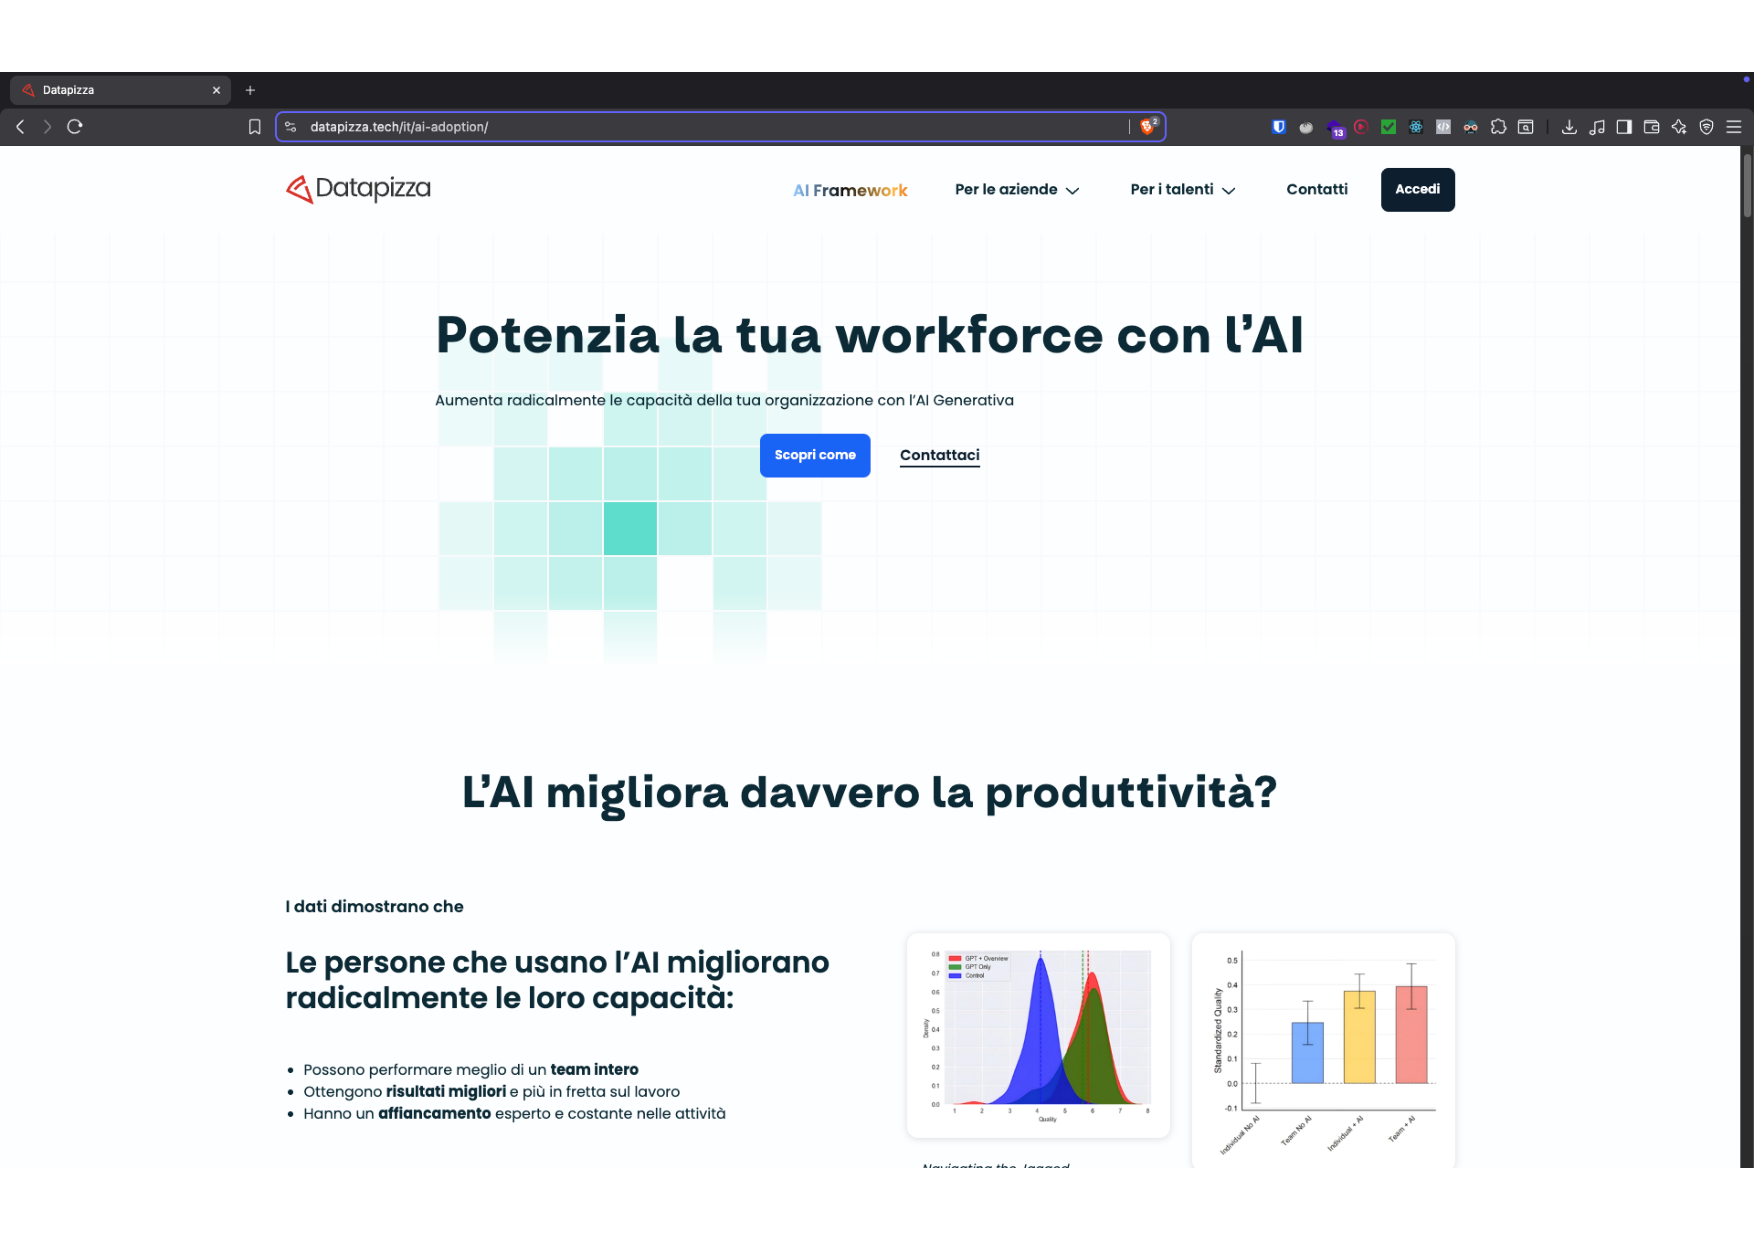
\includegraphics[width=\textwidth]{chapters/figures/landingAI.pdf}
    \caption{Screenshot della landing AI Adoption in versione desktop.}
    \label{fig:landing-desktop}
\end{figure}

\clearpage

\begin{figure}[h!]
    \centering
    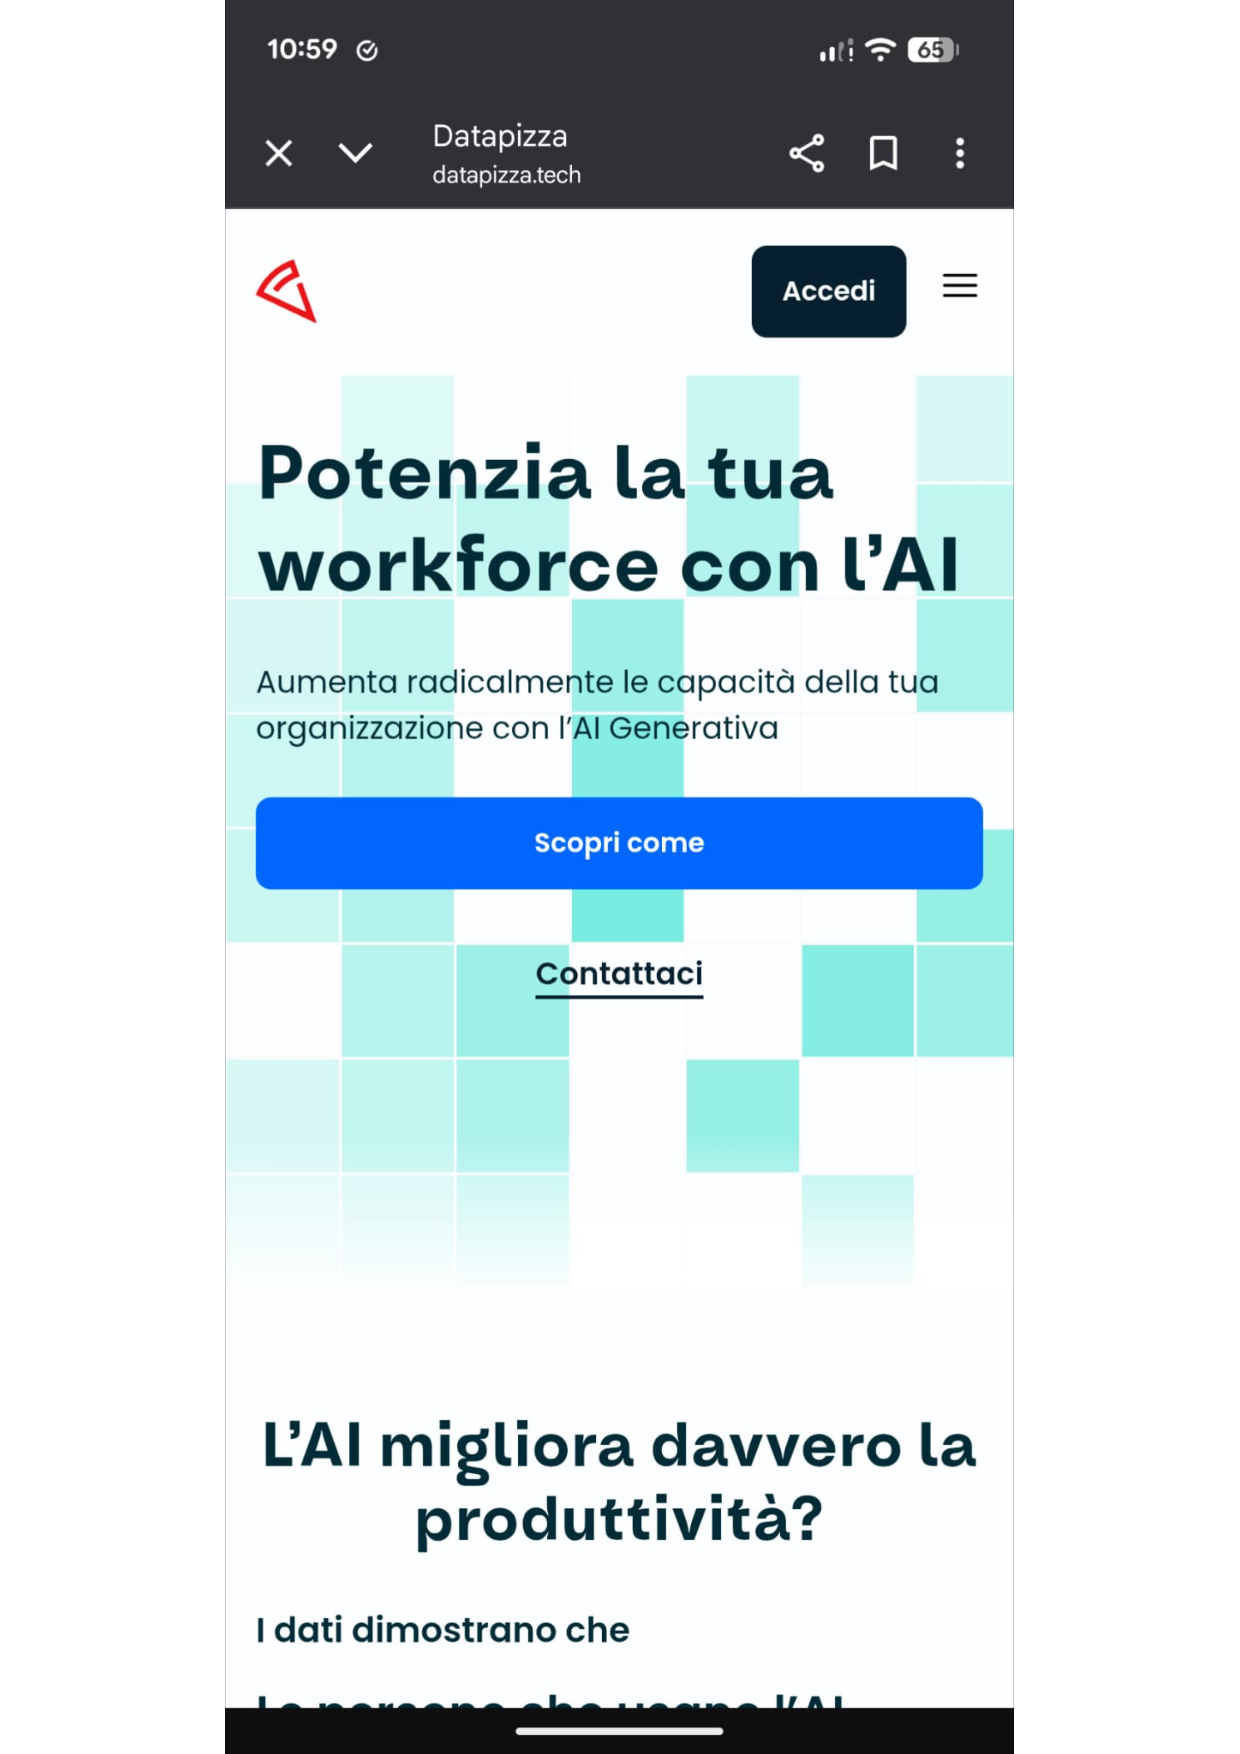
\includegraphics[width=0.5\textwidth]{chapters/figures/landingAImobile.pdf}
    \caption{Screenshot della landing AI Adoption in versione mobile.}
    \label{fig:landing-mobile}
\end{figure}

\section{Criticità post-lancio e risoluzione}

Nelle prime settimane dopo il rilascio è emersa una problematica sui form di 
contatto delle landing B2B: il sistema registrava doppi invii causando lead 
duplicati nel CRM del team sales. L'analisi ha rivelato che il pulsante "Invia" 
non si disabilitava immediatamente, permettendo click multipli durante il 
processing, e mancava feedback visivo chiaro post-submit.

La risoluzione ha implementato la disabilitazione automatica del pulsante al 
primo click e un alert di conferma esplicito che comunica l'avvenuto 
completamento. Il deployment completato in una settimana ha eliminato 
completamente i doppi invii. Questo incident ha consolidato best practices 
per sviluppi futuri: testing con scenari stress, feedback visivo obbligatorio 
fin dal design, e monitoring granulare post-deploy.

\section{Tracking e monitoraggio}

Il sistema di tracking Mixpanel implementato permette di monitorare il customer 
journey completo attraverso funnel di conversione differenziati per verticale. 
La Figura \ref{fig:mixpanel-dashboard} mostra un esempio di dashboard analytics 
che evidenzia le metriche di engagement e i punti di drop-off nel percorso utente, 
abilitando ottimizzazioni data-driven delle landing pages.

\begin{figure}[h!]
    \centering
    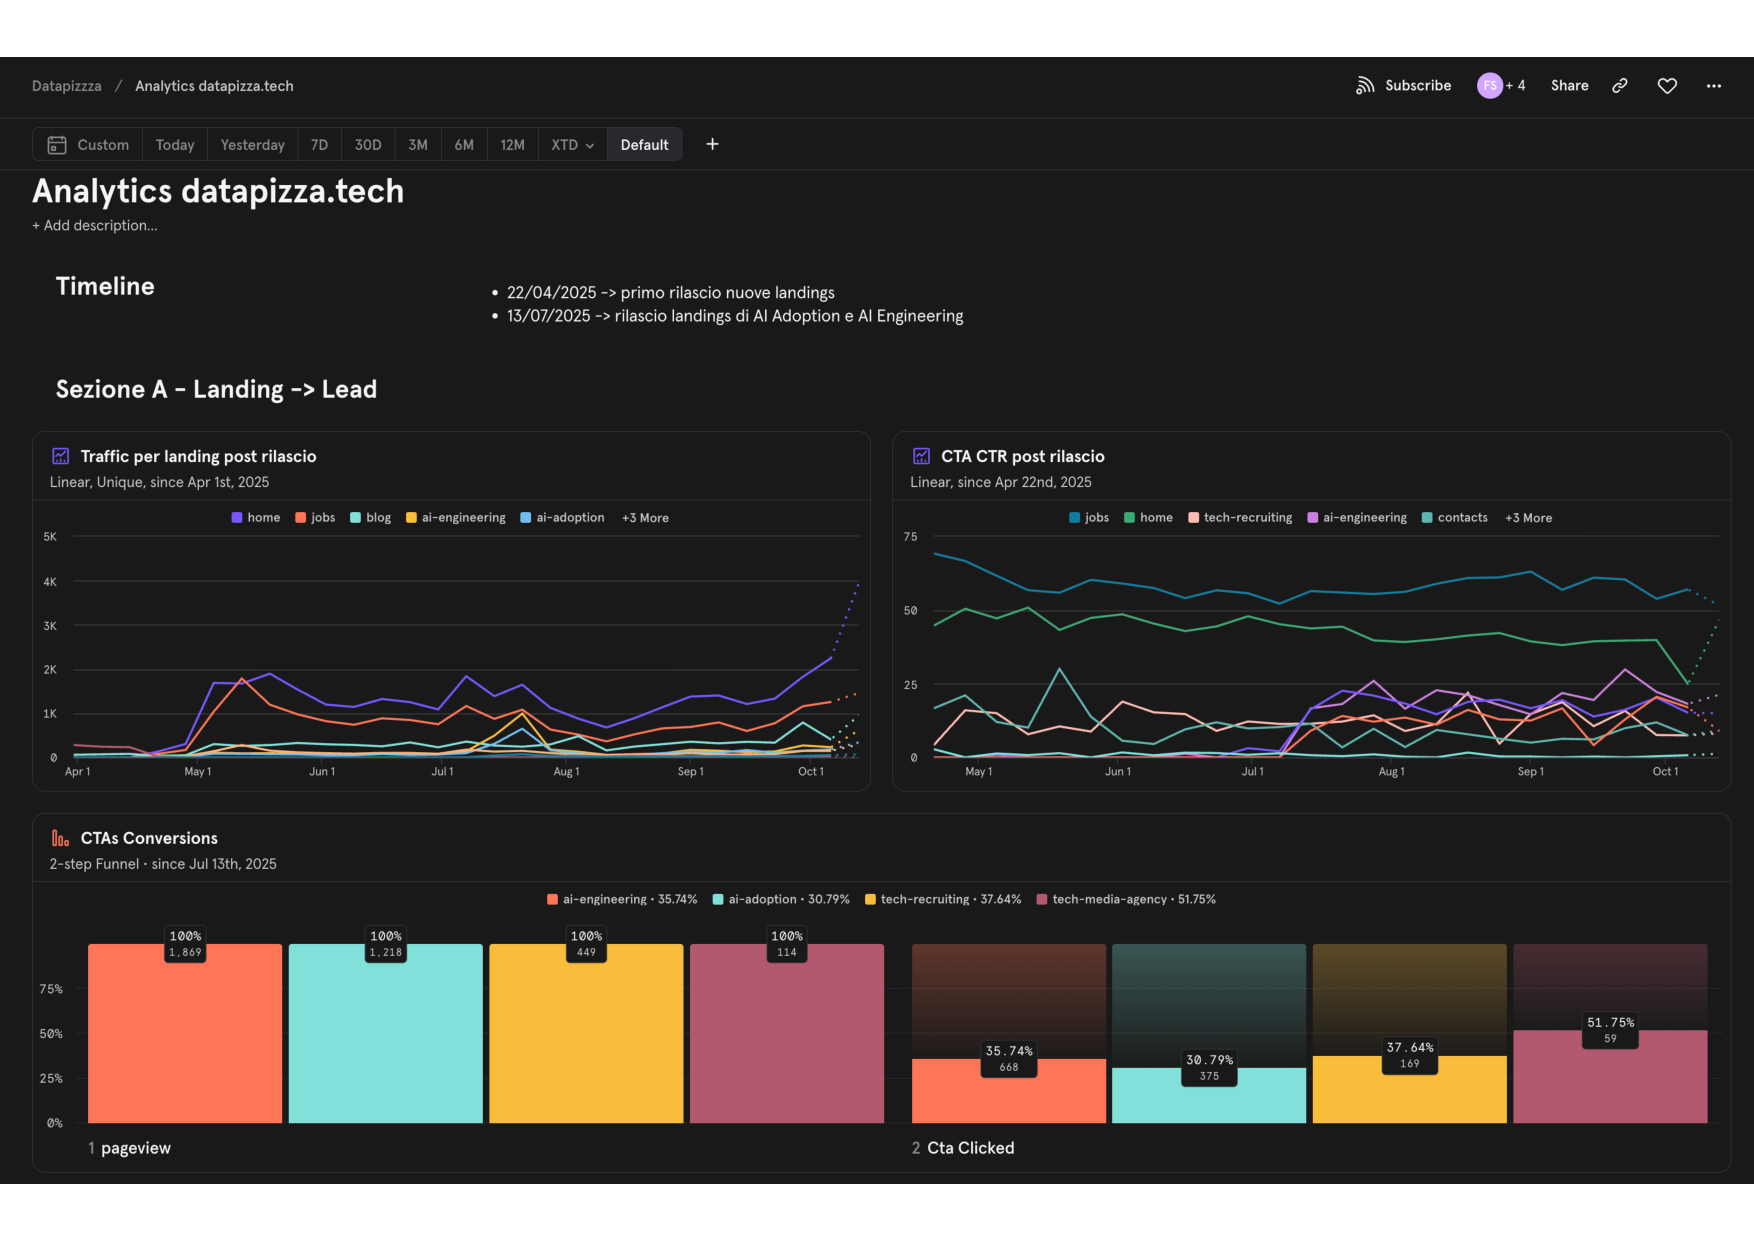
\includegraphics[width=\textwidth]{chapters/figures/metriche1.pdf}
    \caption{Dashboard Mixpanel che mostra funnel di conversione e metriche 
    di engagement per analisi data-driven.}
    \label{fig:mixpanel-dashboard}
\end{figure}

\section{Risultati complessivi}

Il progetto ha raggiunto gli obiettivi tecnici e di business definiti nei 
capitoli precedenti. Le performance sono state ottimizzate su tutti i dispositivi, 
l'accessibilità è verificata conformemente agli standard WCAG 2.1 livello AA, 
e le ottimizzazioni SEO hanno garantito indicizzazione corretta su tutti i motori 
di ricerca. L'architettura modulare implementata garantisce scalabilità concreta 
con tempo stimato di 2-4 settimane per sviluppare nuove landing verticali 
riutilizzando i componenti esistenti.

Le landing pages hanno abilitato il posizionamento chiaro dei quattro verticali 
aziendali con messaggi differenziati per target B2B e B2C. Il sistema di tracking 
fornisce al team marketing visibilità completa sui funnel di conversione, 
permettendo ottimizzazioni continue basate su dati reali.

\bigskip
Il progetto ha fornito una base scalabile e performante per la crescita futura, 
validando l'approccio multi-landing con architettura modulare riutilizzabile.